\clearpage
\section{Příklady z minulých zkoušek}
\subsection{Zadání 1}
\begin{enumerate}
    \item \textbf{Vypočtěte amplitudu základní(1.) harmonické složky unipolárního signálu RZ při bitové posloupnosti ...101010... Doba trvání impulzu je poloviční oproti době trvání bitu. Výška impulzu je 5V}
    \begin{align*}
        C_1 = 2\cdot D \cdot \frac{\vartheta}{T_0}\cdot sinc(\frac{\vartheta}{2}\cdot\frac{2\pi}{T_0}) = \frac{10}{4} \cdot \frac{sin(\frac{\vartheta}{2}\cdot\frac{2\pi}{4\vartheta})}{\frac{\vartheta}{2}\cdot\frac{2\pi}{4\vartheta}} =  2,2508V
    \end{align*}
    \item \textbf{Jakou minimální kmitočtovou šířku pásma propustnosti potřebuje pro přenos signálu FSK, je-li \(f_1 = 100 kHz\), \(f_0 = 105 kHz\) a data mají být přenášena rychlostí R=5kbit/s.}
    \begin{align*}
        B_{min} = \left | f_0 - f_1 \right | + M \\
        B_{min} = \left | f_0 - f_1 \right | + R \\ 
        B_{min} = 10kHz
    \end{align*}
    V tomto případě se M = R. 
    
    \item \textbf{Blokové schéma modulátoru QPSK}
    \begin{figure}[h]
        \centering
        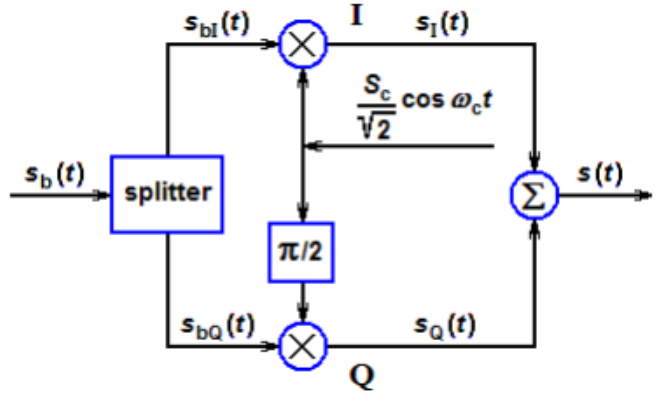
\includegraphics[scale = 0.5]{images/QPSK.png}
        \caption{Modulátor}
        \label{fig:enter-label}
    \end{figure}
    \item \textbf{Je dán modulátor 256QAM. Kolika stavový signál je v kanálu I a v kanálu Q?}\
    \begin{align*}
        L_I = L_Q = \sqrt{Q} = \sqrt{256} = 16
    \end{align*}
    Počet stavů signálu v kanálu Q a I je 16
    \item \textbf{Bipolární signál NRZ s napěťovými úrovněmi +5V a -5V je zarušen normálním šumem s
    efektivní hodnotou napětí 1,5V. Pravděpodobnost výskytu log. nuly a jedničky jsou stejné.
    Stanovte pravděpodobnost \(P_E\) chybného příjmu.}
    \begin{align*}
        P_E = F_0(\frac{D_0 - D_1}{2\sigma}) = F_0(-3,33) = 4.3423\cdot10^{-4}
    \end{align*}
    \item \textbf{Nakreslete časový průběh bipolárního signálu NRZ vyjadřujícího dat. posloupnost 10110 a
    odpovídající odezvu přizpůsobeného filtru.}
    \begin{figure}[h]
        \centering
        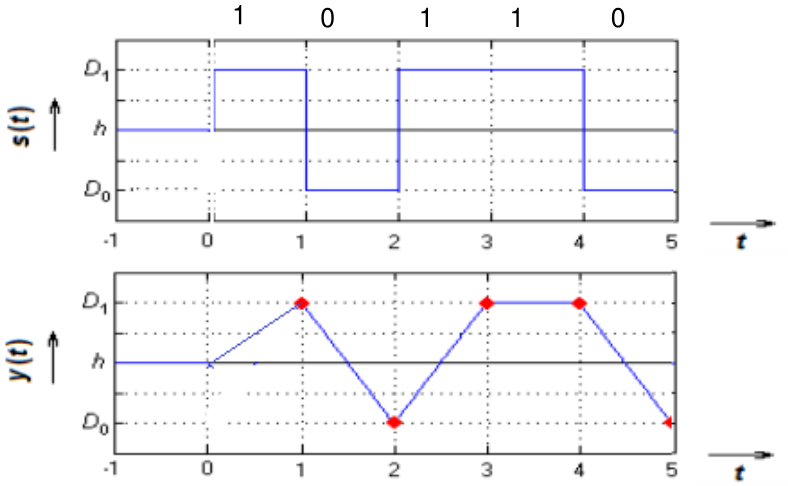
\includegraphics[scale = 0.5]{images/NRZfiltr.png}
        \caption{Průběh a odezva}
        \label{fig:enter-label}
    \end{figure}
    \item \textbf{Jaký je účel interleavingu (prokládání), v čem spočívá jeho princip, jakým negativním jevem
    je provázen?}
    \begin{itemize}
        \item Ochrana proti chybám zapříčiněných opakovanými stejnými znaky (0000000000, 1111111) a
        vznikajícími přenosem kanálem.
        \item Jednotlivé bity jsou po výstupu z kodéru pro dopředné potlačení chyb zpožděny o různý čas.
        \item Shluk chyb je rozprostřen, izolované chyby lze opravit.
    \end{itemize}
    \item \textbf{Jak závisí index kmitočtové modulace \(\beta\) na kmitočtu modulačního signálu F a
    kmitočtovém zvdihu \(\Delta f\)?}
    \begin{align*}
        \beta = \frac{\Delta f}{F}
    \end{align*}
    \item \textbf{Signál v základním pásmu je tvořen signálovými prvky linkového kódu 2B1Q s dobou
    trvání \(T_s = 250 \mu s\). Stanovte přenosovou rychlost R a modulační rychlost M.}
    \begin{align*}
        M = \frac{1}{T_s} = \frac{1}{250 \cdot 10^{-6}} = 4kBd\\
        M = \frac{R}{2} \Rightarrow R = 2\cdot M = 8kbit/s
    \end{align*}
    \item \textbf{Do připraveného grafu zakreslete modulové kmit. charakteristiky Nyquistova filtru (raised
    cosine filter) pro následující hodnoty činitele tvaru (roll off factor) \(\alpha = 0, \alpha = 0,5, \alpha = 1\)}
    \begin{figure}[h]
        \centering
        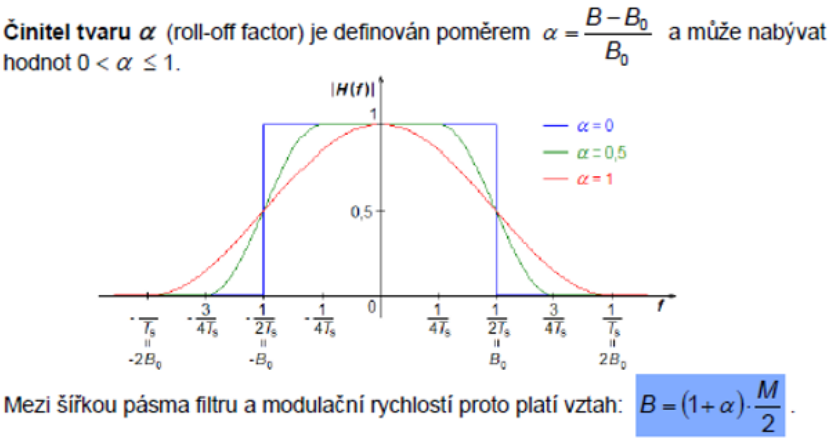
\includegraphics[scale = 0.5]{images/NyquistFilter.png}
        \caption{Nyquistův filter}
        \label{fig:enter-label}
    \end{figure}
\end{enumerate}

\subsection{Zadání 2}
\begin{enumerate}
    \item \textbf{Jaký musí být minimální vzorkovací kmitočet kodéru delta modulace, aby nedošlo k jeho
    přetížení, je-li maximální strmost modulačního signálu max [f`(t)] = 800V/s a kvantizační
    krok \(\Delta s = 40mV\)?}
    \begin{align*}
        f_{vz} = \frac{A}{\Delta s} = \frac{800}{0,04} = 20kHz
    \end{align*}
    \item \textbf{Jaký druh klíčování realizuje modulátor na následujícím obrázku? O kolik stupňů nebo
    radiánů se může měnit počáteční fáze takto klíčovaného signálu na rozhraní sousedních
    sign. prvků? Pozn. uvést všechny možné hodnoty.}\\
    \begin{figure}[h]
        \centering
        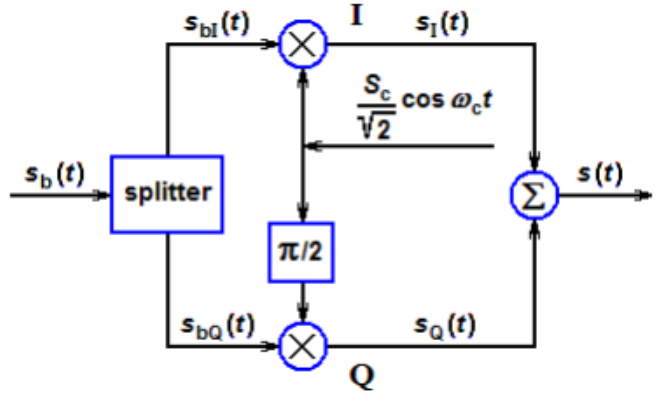
\includegraphics[scale = 0.3]{images/QPSK}
        \caption{Modulátor}
        \label{fig:enter-label}
    \end{figure}\\
    Je to QPSK. Počáteční fáze na rozhraní sousedních signálových prvků se mohou měnit o \(\pm \frac{pi}{2} = \pm 90^{\circ}\).
    \item \textbf{Nakreslete časový průběh bipolárního NRZ vyjadřujícího datovou posloupnost 10110 a
    odpovídající odezvu vybíjeného integrátoru.}
    \begin{figure}[h]
        \centering
        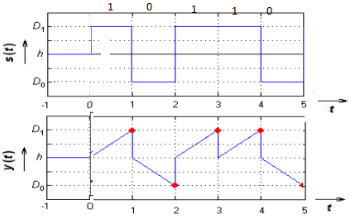
\includegraphics[scale = 0.7]{images/VybInteg.png}
        \caption{Průběh a odezva}
        \label{fig:enter-label}
    \end{figure}
    \item \textbf{Je dán kvadraturní modulátor MQAM. Kanál I má 8 stavů, kanál Q má také 8 stavů. Kolik
    bitů vyjadřuje jeden signálový prvek výsledného modulovaného signálu na výstupu modulátoru.}
    \begin{align*}
        M-QAM \Rightarrow M = I\cdot Q = 64\\
        N = log_{2}(M) = log_{2}(64) = 6
    \end{align*}
    \item \textbf{Jaká je hlavní nevýhoda systému DPCM?}\\
    Kumulace chyb
    \item \textbf{Modulovaný signál je popsán rovnicí \(s(t) = S_c cos(\omega_c \cdot t+ \varphi\cdot f(t))\), kde \(f(t)\) je normovaný modulační signál. O jaký druh modulace se jedná? Co vyjadřuje konstanta \(\Delta \varphi\)?}\\
    Jde o fázovou modulaci PM. Kde \(\Delta \varphi\) vyjadřuje fázový zdvih.
    \item \textbf{Kapacita binárního kanálu je C = 0,6 Sh/znak. Stanovte kapacitu C' (maximum vzájemné
    informace přenesené za jednotku času), je-li horní mezní kmitočet kanálu chápaného jako
    dolní propust \(f_h = 500Hz\)}
    \begin{align*}
        C' = 2 \cdot f_h \cdot C = 600Sh/znak
    \end{align*}
    \item \textbf{Nakreslete blokové schéma modulátoru sigma–delta}
    \begin{figure}[h]
        \centering
        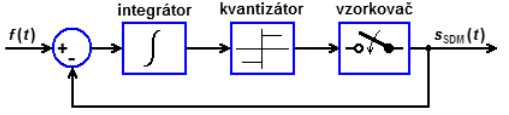
\includegraphics[scale = 0.7]{images/SDM.png}
        \caption{Sigma-Delta modulátor}
        \label{fig:enter-label}
    \end{figure}
    \item \textbf{Bipolárním signálem RZ o napěťových úrovních +1V a -1V je přenášena periodická datová
    posloupnost 110110110 Doba trvání impulzu \(\vartheta\) je poloviční oproti trvání bitu,
    která je \(T_b = 250 \mu s\). Určete ss složku signálu a přenosovou rychlost.}
    \begin{align*}
        A_0 = D\cdot\frac{p\vartheta - n\vartheta}{T_0} = 1\frac{1}{6} = 0,1667V\\
        M = \frac{1}{T_s} = 8kBd = 2\cdot R \Rightarrow R = \frac{M}{2} = 4kbit/s
    \end{align*}
    \item \textbf{Do připraveného grafu zakreslete spektrum amplitud signálu BPSK, který přenáší
    periodickou datovou posloupnost 010101. Rychlostí 10kbit/s. Amplituda nosného signálu je
    \(S_c=1V\) a kmitočet \(f_c = 30kHz\).}\\
    \(M = R \Rightarrow B_{min} = M = 10kHz \Rightarrow F = \frac{M}{2} = 5kHz\). Rozestupy mezi harmonickými budou 5kHz.\\
    \begin{figure}[h]
        \centering
        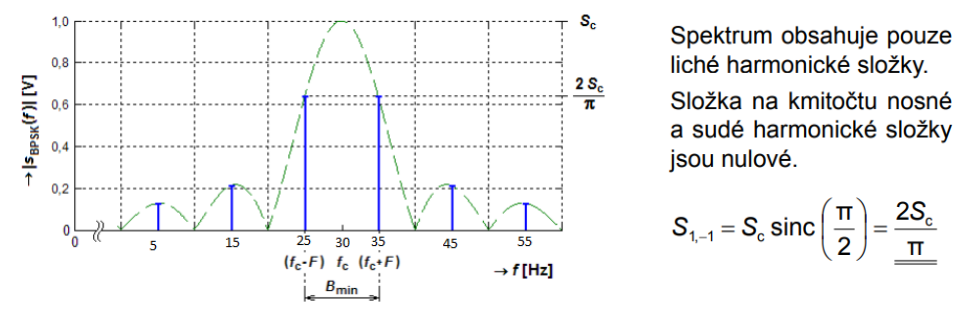
\includegraphics[scale = 0.4]{images/BPSK.png}
        \caption{Spektrum BPSK}
        \label{fig:enter-label}
    \end{figure}

\end{enumerate}
